\documentclass[10pt, letterpaper]{amsart}
\usepackage{pdfpages}

\begin{document}

\begin{figure}[!htbp]
  \caption{Scatter plot matrix for all variables}
  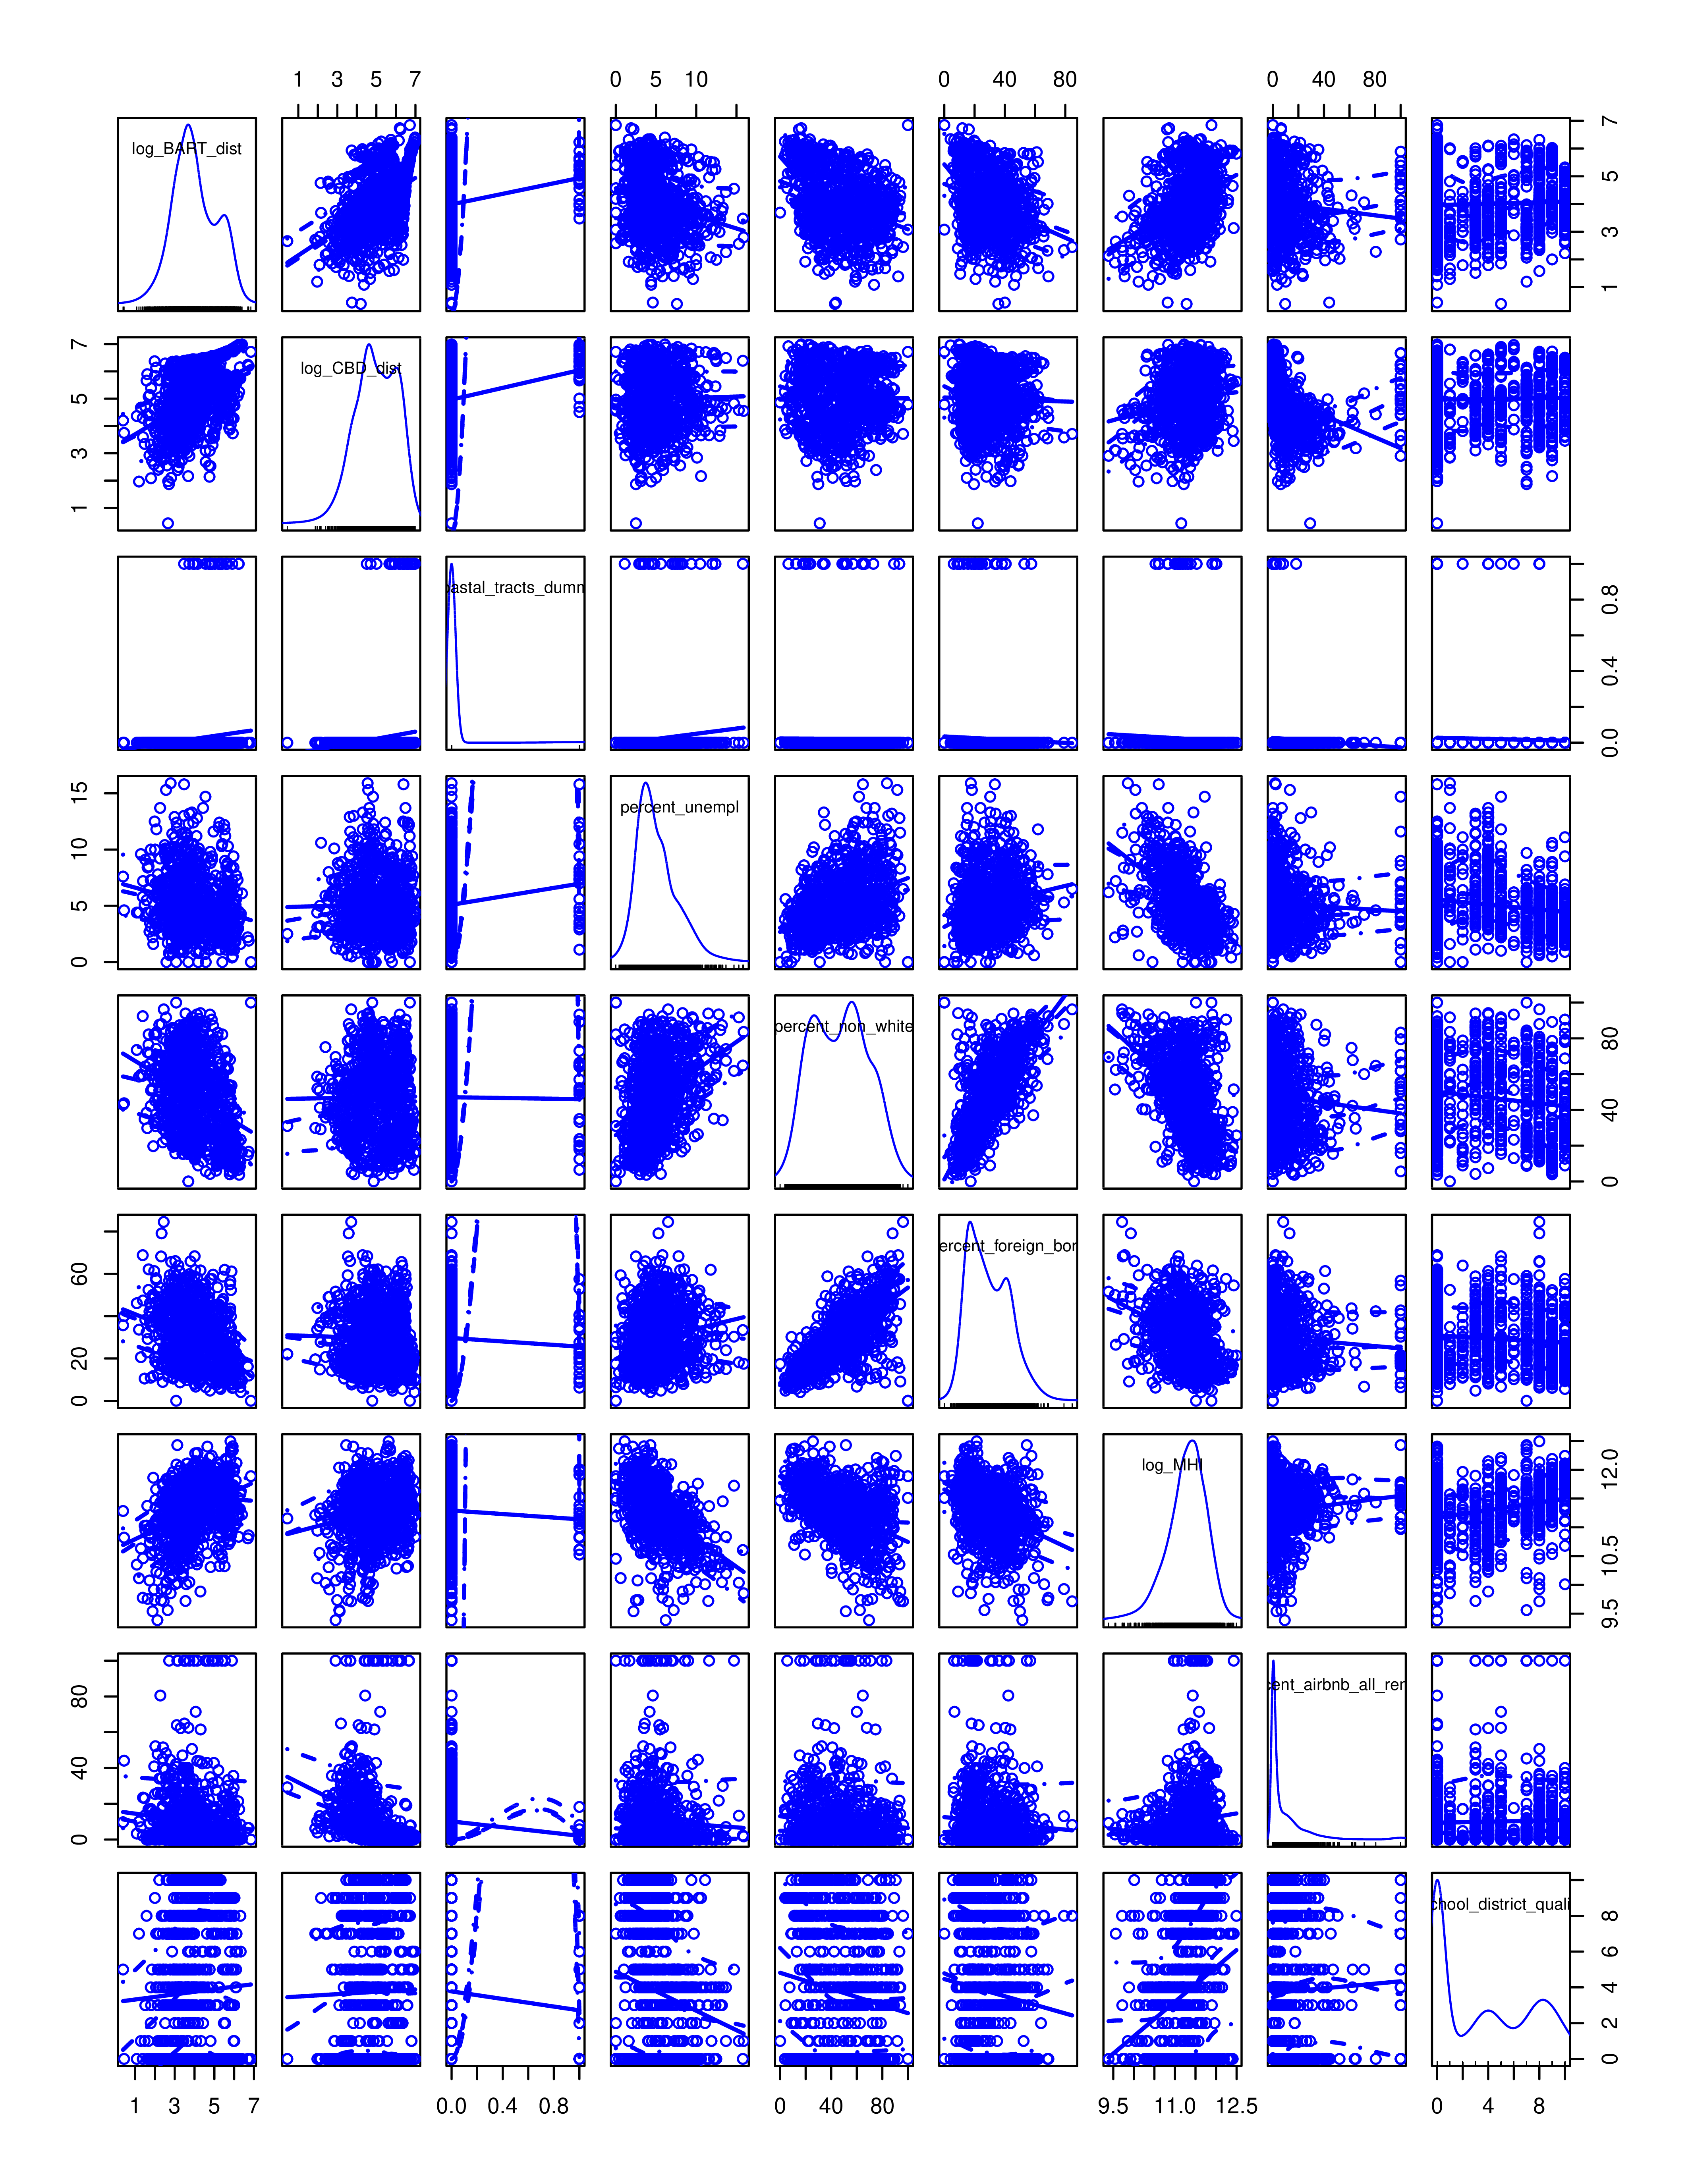
\includegraphics[scale=0.6]{Scatter_plot_matrix_all_variables}
\end{figure}

\begin{figure}[!htbp]
  \caption{Scatter plot matrix for selected variables}
  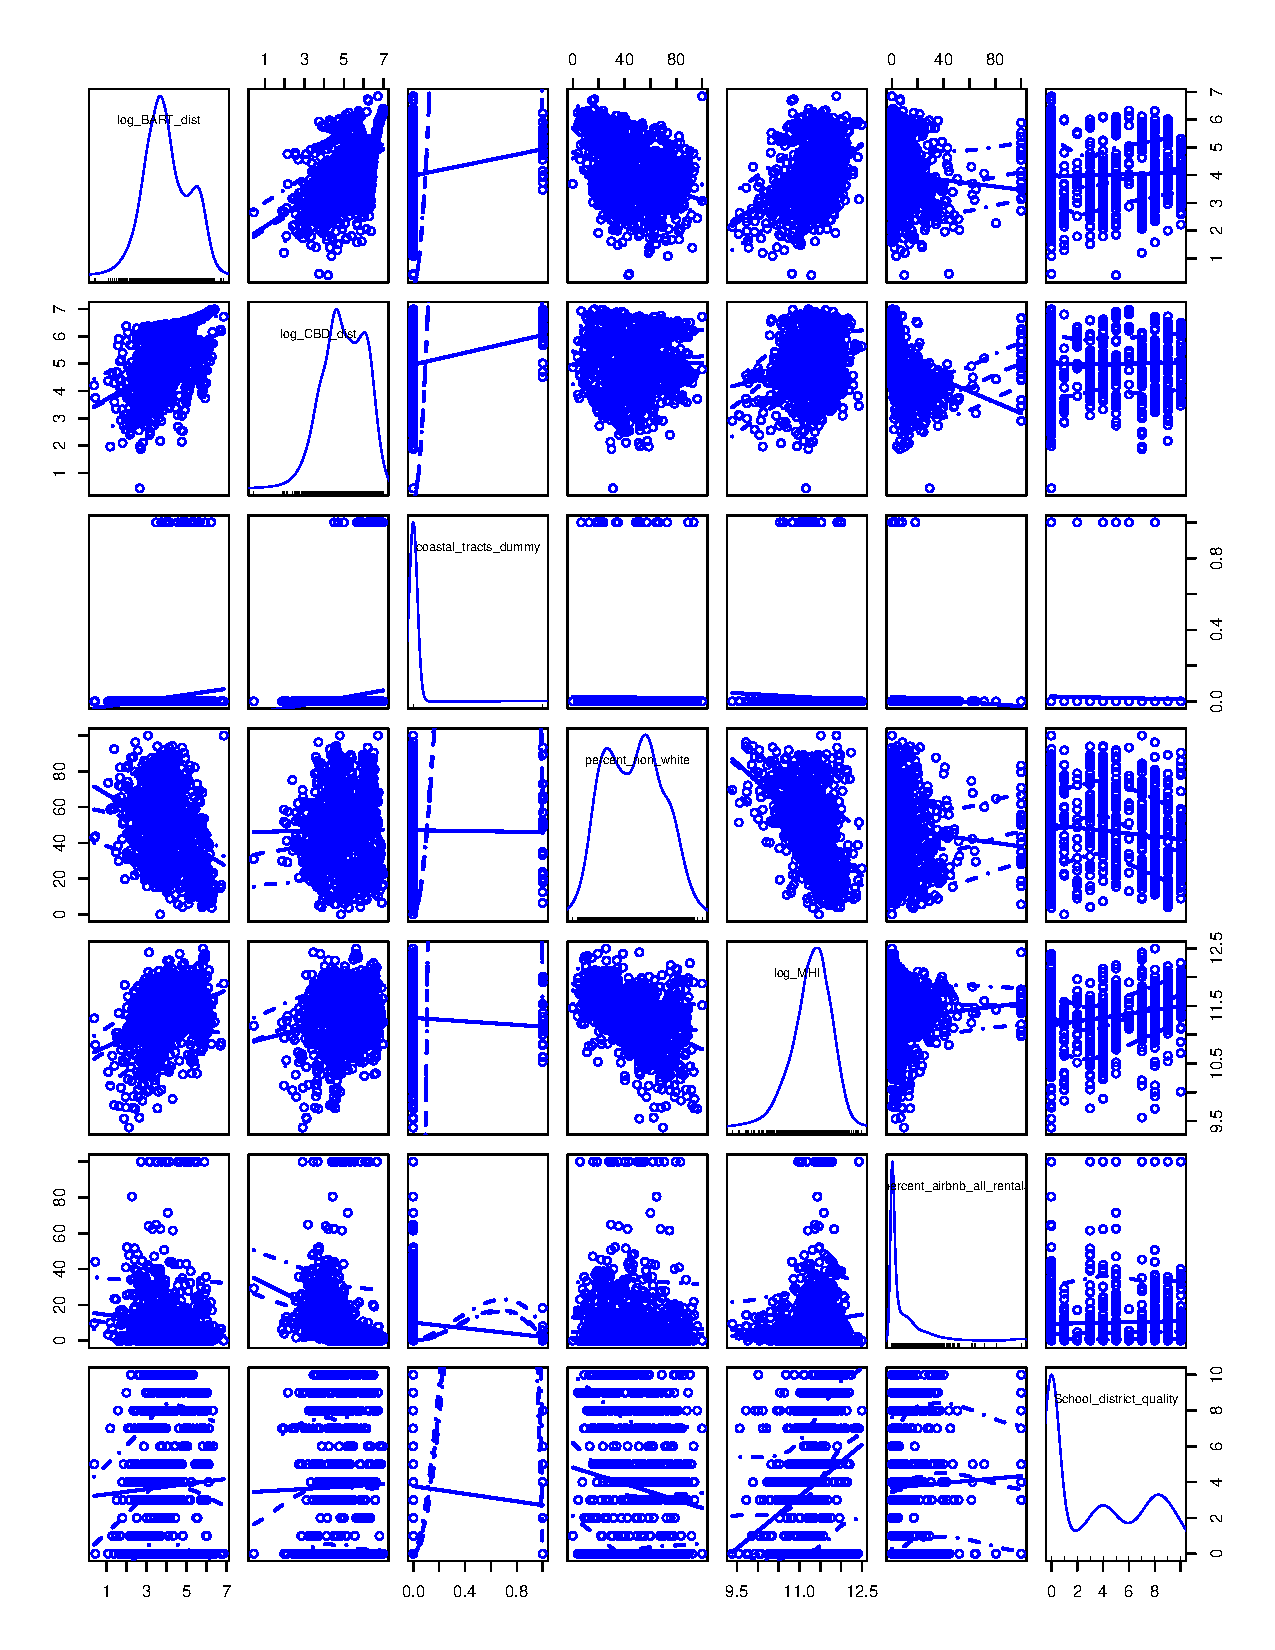
\includegraphics[scale=0.6]{Scatter_plot_matrix_selected_variables}
\end{figure}

\begin{figure}[!htbp]
  \caption{Spatial Weights (neighbors)}
  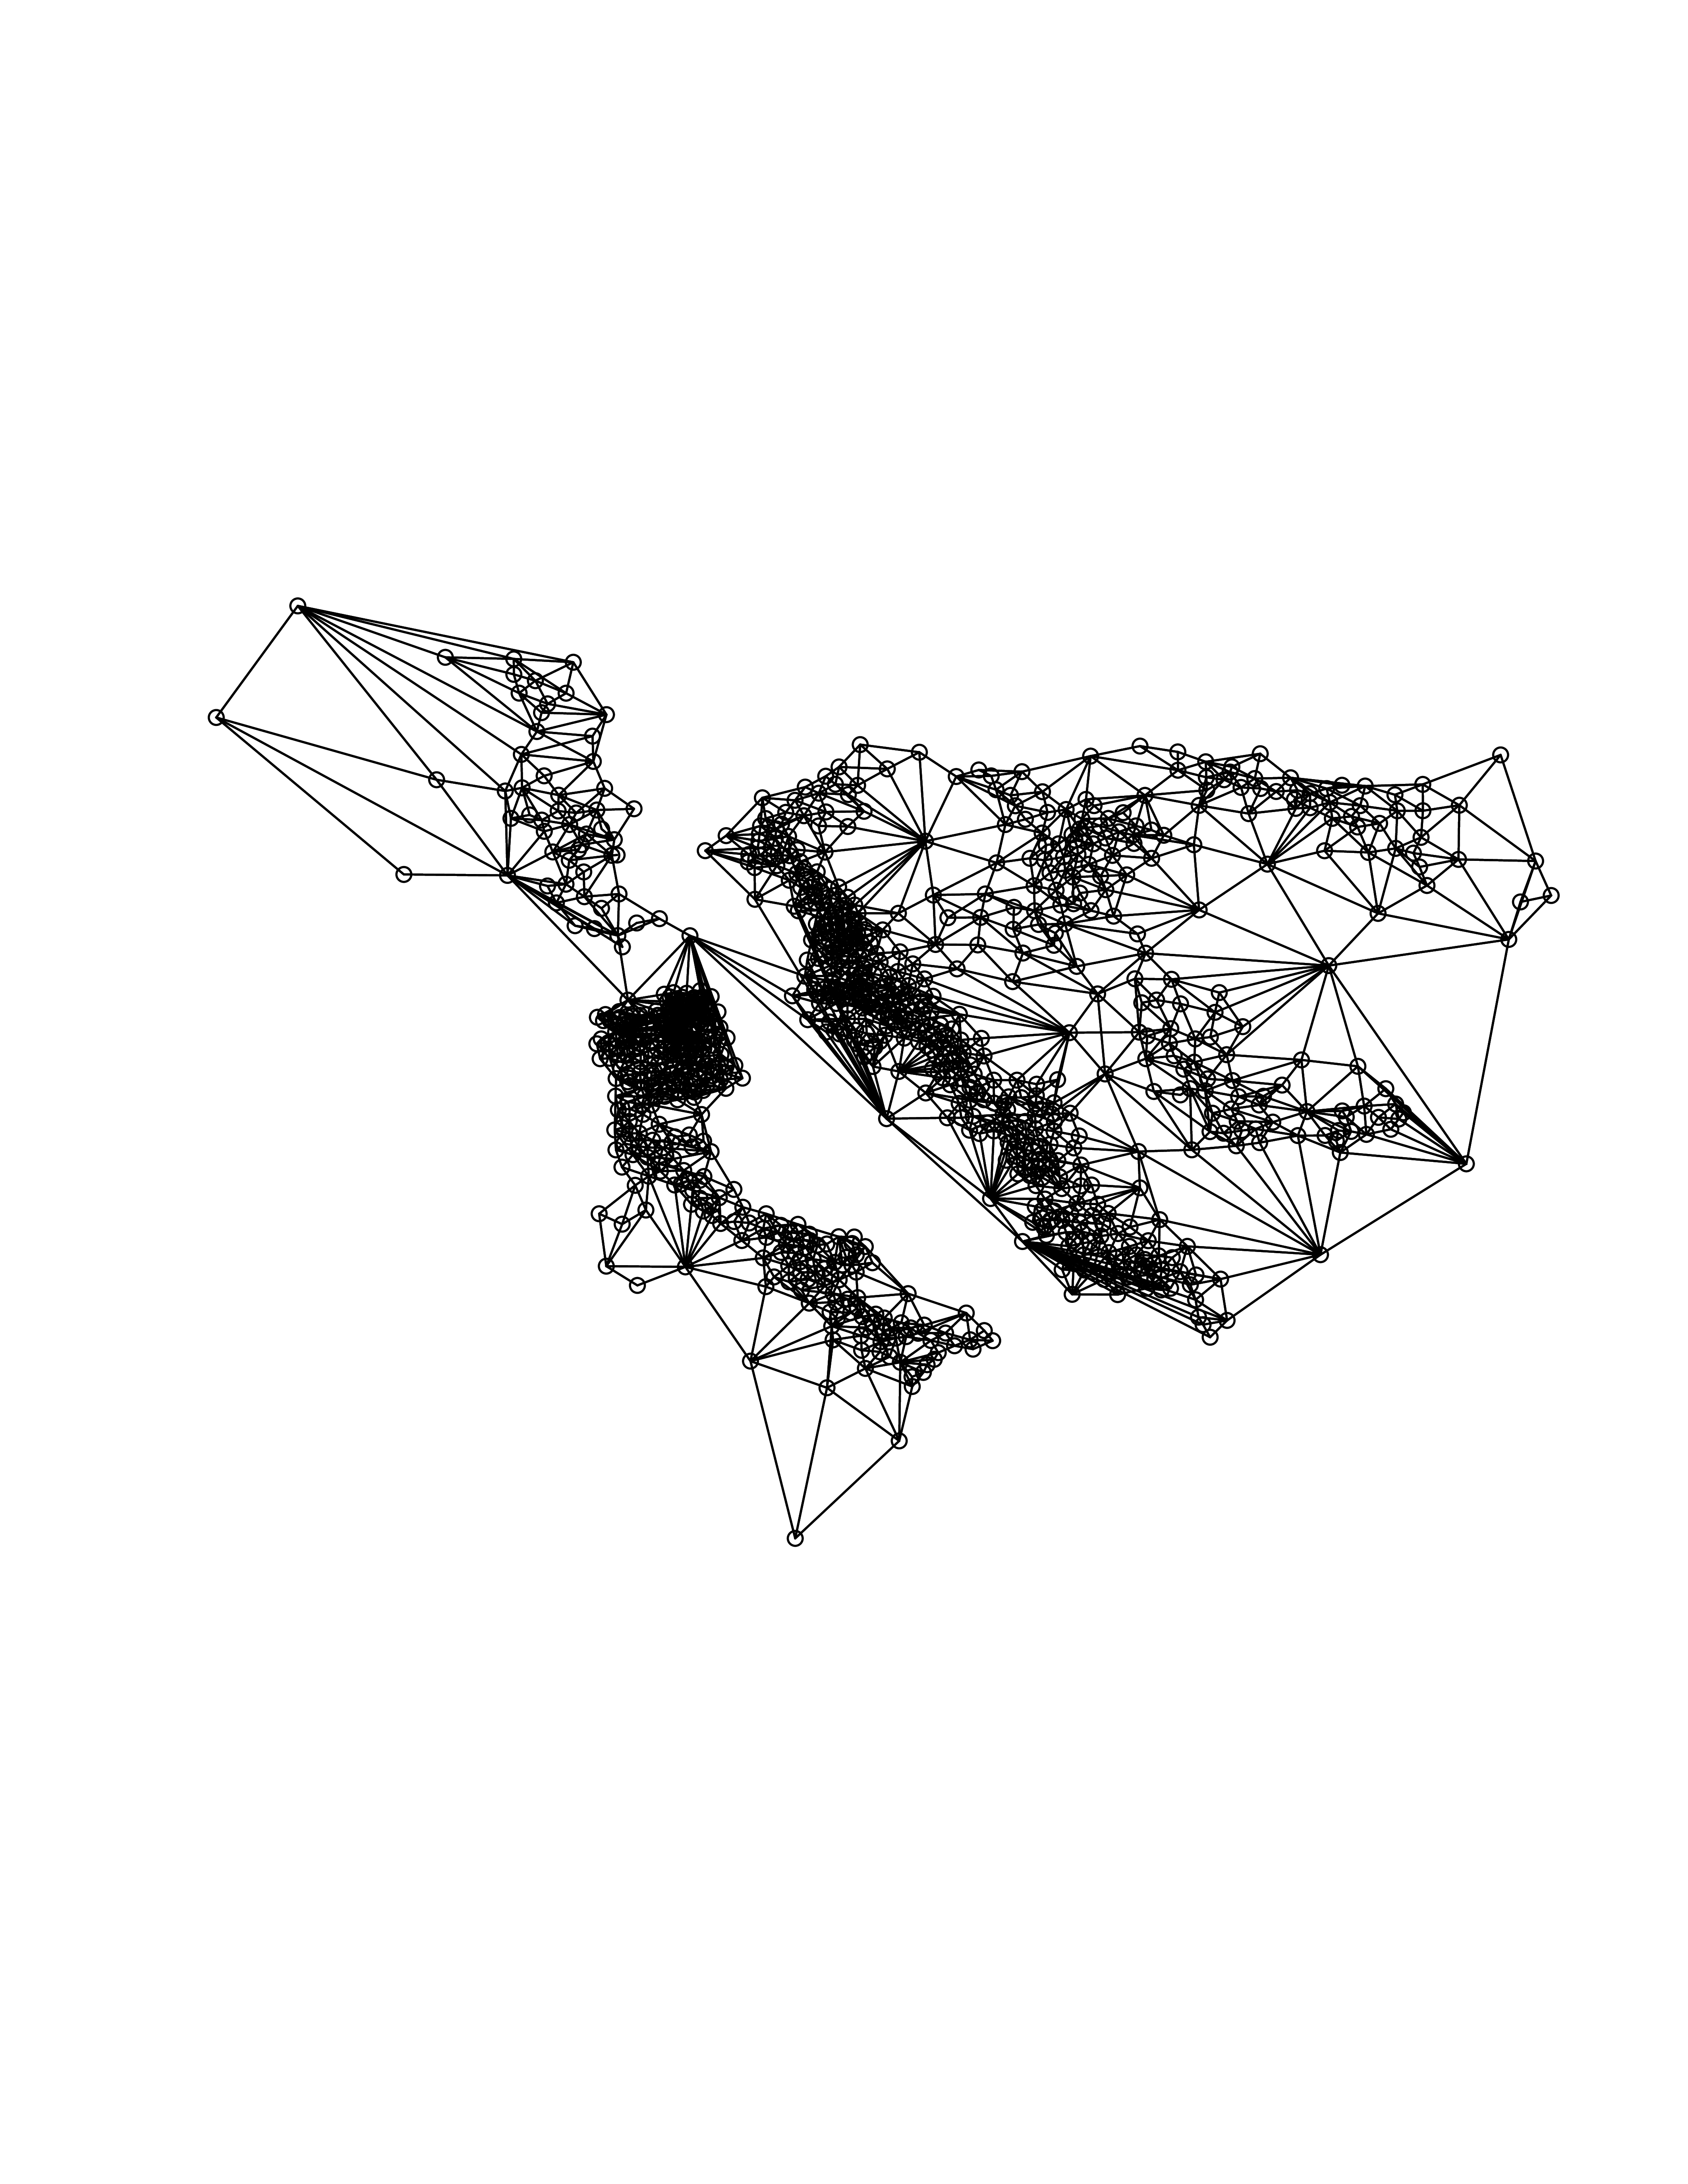
\includegraphics[scale=0.1]{Spatial_Weight_Matrix}
\end{figure}


% Table created by stargazer v.5.2 by Marek Hlavac, Harvard University. E-mail: hlavac at fas.harvard.edu
% Date and time: Thu, May 24, 2018 - 05:42:57 PM
\begin{table}[!htbp] \centering 
  \caption{Regression: selected variables} 
  \label{} 
  \begin{tabular}{@{\extracolsep{5pt}}lc} 
    \\[-1.8ex]\hline 
    \hline \\[-1.8ex] 
    & \multicolumn{1}{c}{\textit{Dependent variable:}} \\ 
    \cline{2-2} 
    \\[-1.8ex] & rent\_burdened \\ 
    \hline \\[-1.8ex] 
    log\_BART\_dist & 1.542$^{***}$ \\ 
    & (0.407) \\ 
    & \\ 
    log\_CBD\_dist & 2.437$^{***}$ \\ 
    & (0.418) \\ 
    & \\ 
    coastal\_tracts\_dummy & $-$4.571$^{*}$ \\ 
    & (2.565) \\ 
    & \\ 
    percent\_non\_white & 0.045$^{**}$ \\ 
    & (0.020) \\ 
    & \\ 
    log\_MHI & $-$16.684$^{***}$ \\ 
    & (0.926) \\ 
    & \\ 
    percent\_airbnb\_all\_rentals & 0.059$^{***}$ \\ 
    & (0.022) \\ 
    & \\ 
    School\_district\_quality & 0.073 \\ 
    & (0.103) \\ 
    & \\ 
    Constant & 214.067$^{***}$ \\ 
    & (10.302) \\ 
    & \\ 
    \hline \\[-1.8ex] 
    Observations & 975 \\ 
    R$^{2}$ & 0.328 \\ 
    Adjusted R$^{2}$ & 0.323 \\ 
    Residual Std. Error & 11.404 (df = 967) \\ 
    F Statistic & 67.426$^{***}$ (df = 7; 967) \\ 
    \hline 
    \hline \\[-1.8ex] 
    \textit{Note:}  & \multicolumn{1}{r}{$^{*}$p$<$0.1; $^{**}$p$<$0.05; $^{***}$p$<$0.01} \\ 
  \end{tabular} 
\end{table}

% Table created by stargazer v.5.2 by Marek Hlavac, Harvard University. E-mail: hlavac at fas.harvard.edu
% Date and time: Thu, May 24, 2018 - 05:45:43 PM
\begin{table}[!htbp]
  \caption{VIF: check ofr multicollinearity} 
  \label{}
  \hspace*{-4.5cm}
  \begin{tabular}{@{\extracolsep{5pt}} ccccccc} 
    \\[-1.8ex]\hline 
    \hline \\[-1.8ex] 
    log\_BART\_dist & log\_CBD\_dist & coastal\_tracts\_dummy & percent\_non\_white & log\_MHI & percent\_airbnb\_all\_rentals & School\_district\_quality \\ 
    \hline \\[-1.8ex] 
    $1.539$ & $1.494$ & $1.039$ & $1.402$ & $1.515$ & $1.164$ & $1.075$ \\ 
    \hline \\[-1.8ex] 
  \end{tabular} 
\end{table} 








% Table created by stargazer v.5.2 by Marek Hlavac, Harvard University. E-mail: hlavac at fas.harvard.edu
% Date and time: Thu, May 24, 2018 - 06:00:47 PM
\begin{table}[!htbp] \centering 
  \caption{OLS regression: selected variables} 
  \label{} 
  \begin{tabular}{@{\extracolsep{5pt}}lc} 
    \\[-1.8ex]\hline 
    \hline \\[-1.8ex] 
    & \multicolumn{1}{c}{\textit{Dependent variable:}} \\ 
    \cline{2-2} 
    \\[-1.8ex] & Y \\ 
    \hline \\[-1.8ex] 
    Xlog\_BART\_dist & 1.542$^{***}$ \\ 
    & (0.407) \\ 
    & \\ 
    Xlog\_CBD\_dist & 2.437$^{***}$ \\ 
    & (0.418) \\ 
    & \\ 
    Xcoastal\_tracts\_dummy & $-$4.571$^{*}$ \\ 
    & (2.565) \\ 
    & \\ 
    Xpercent\_non\_white & 0.045$^{**}$ \\ 
    & (0.020) \\ 
    & \\ 
    Xlog\_MHI & $-$16.684$^{***}$ \\ 
    & (0.926) \\ 
    & \\ 
    Xpercent\_airbnb\_all\_rentals & 0.059$^{***}$ \\ 
    & (0.022) \\ 
    & \\ 
    XSchool\_district\_quality & 0.073 \\ 
    & (0.103) \\ 
    & \\ 
    Constant & 214.067$^{***}$ \\ 
    & (10.302) \\ 
    & \\ 
    \hline \\[-1.8ex] 
    Observations & 975 \\ 
    R$^{2}$ & 0.328 \\ 
    Adjusted R$^{2}$ & 0.323 \\ 
    Residual Std. Error & 11.404 (df = 967) \\ 
    F Statistic & 67.426$^{***}$ (df = 7; 967) \\ 
    \hline 
    \hline \\[-1.8ex] 
    \textit{Note:}  & \multicolumn{1}{r}{$^{*}$p$<$0.1; $^{**}$p$<$0.05; $^{***}$p$<$0.01} \\ 
  \end{tabular} 
\end{table} 


\begin{figure}[!htbp]
  \caption{Moran's I test for spatial autocorrelation -- all variables}
  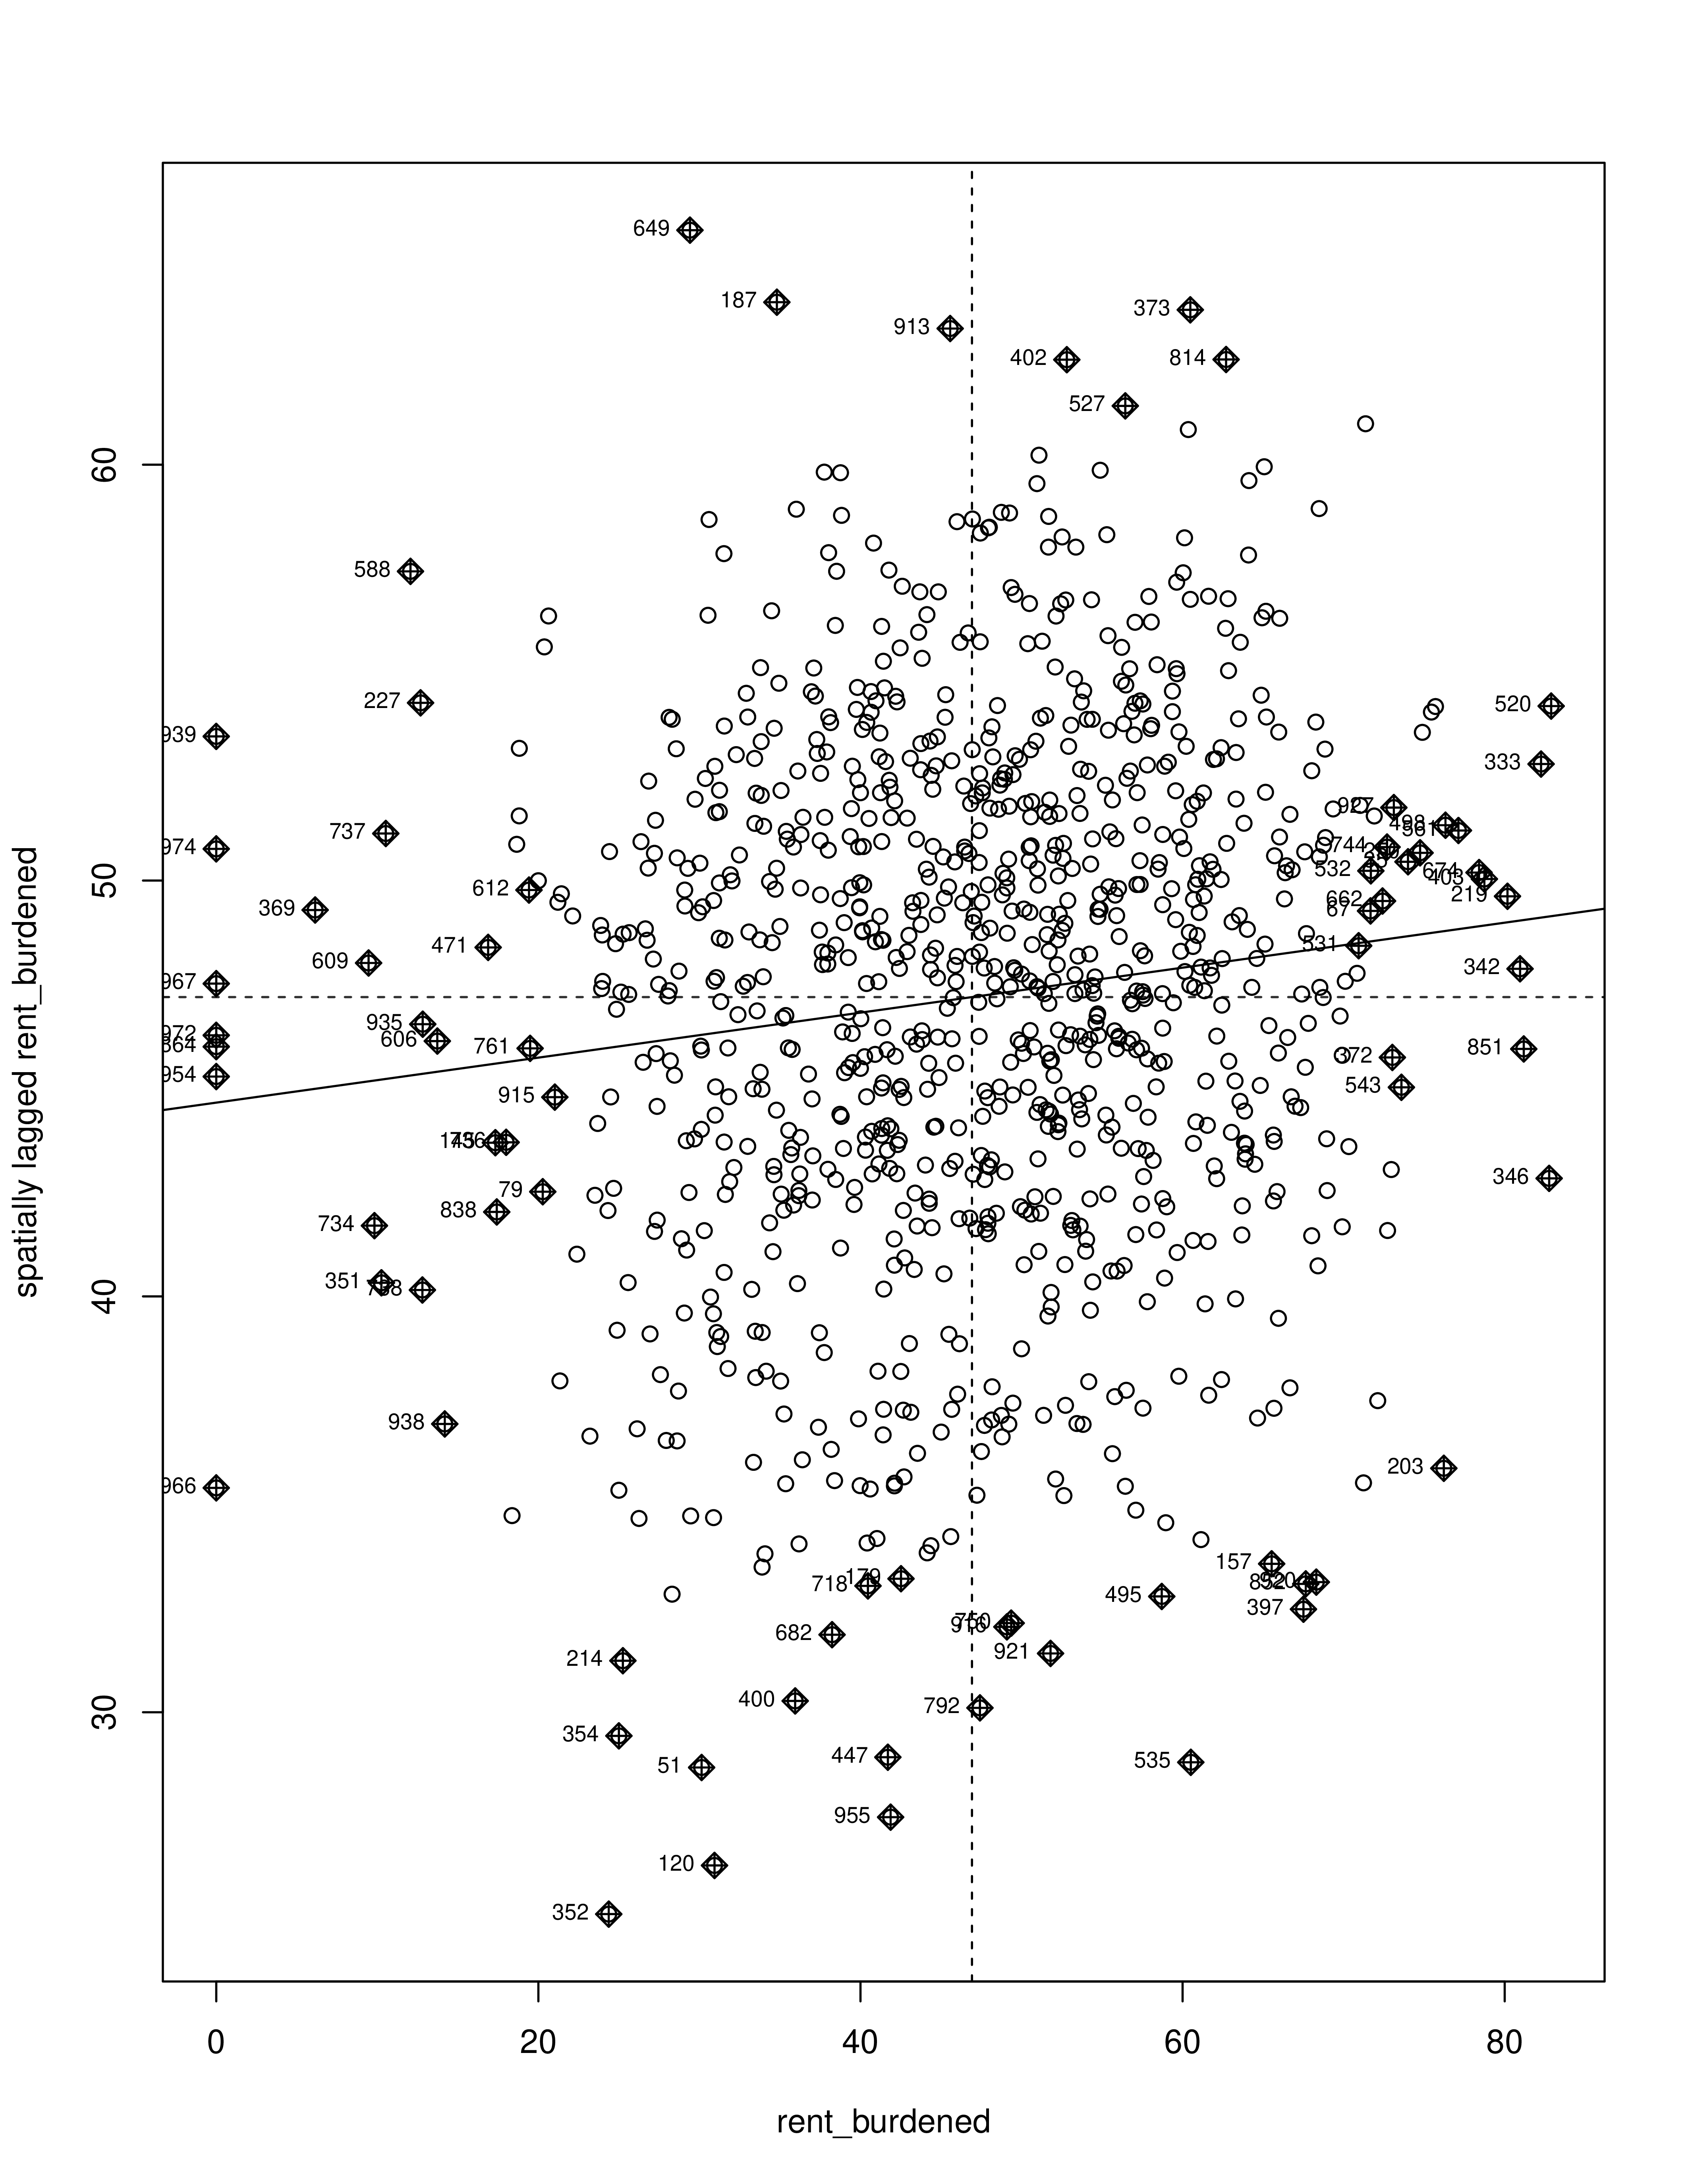
\includegraphics[scale=0.09]{Moran_spatial_autocorrelation_all}
\end{figure}




% Table created by stargazer v.5.2 by Marek Hlavac, Harvard University. E-mail: hlavac at fas.harvard.edu
% Date and time: Thu, May 24, 2018 - 08:44:04 PM
\begin{table}[!htbp] \centering 
  \caption{Spatial Lag Model: selected variables} 
  \label{} 
  \begin{tabular}{@{\extracolsep{5pt}}lc} 
    \\[-1.8ex]\hline 
    \hline \\[-1.8ex] 
    & \multicolumn{1}{c}{\textit{Dependent variable:}} \\ 
    \cline{2-2} 
    \\[-1.8ex] & rent\_burdened \\ 
    \hline \\[-1.8ex] 
    log\_BART\_dist & 1.526$^{***}$ \\ 
    & (0.405) \\ 
    & \\ 
    log\_CBD\_dist & 2.428$^{***}$ \\ 
    & (0.416) \\ 
    & \\ 
    coastal\_tracts\_dummy & $-$4.631$^{*}$ \\ 
    & (2.553) \\ 
    & \\ 
    percent\_non\_white & 0.044$^{**}$ \\ 
    & (0.020) \\ 
    & \\ 
    log\_MHI & $-$16.461$^{***}$ \\ 
    & (0.905) \\ 
    & \\ 
    percent\_airbnb\_all\_rentals & 0.060$^{***}$ \\ 
    & (0.022) \\ 
    & \\ 
    Constant & 210.358$^{***}$ \\ 
    & (10.605) \\ 
    & \\ 
    \hline \\[-1.8ex] 
    Observations & 975 \\ 
    Log Likelihood & $-$3,752.590 \\ 
    $\sigma^{2}$ & 128.967 \\ 
    Akaike Inf. Crit. & 7,523.180 \\ 
    Wald Test & 0.500 (df = 1) \\ 
    LR Test & 0.509 (df = 1) \\ 
    \hline 
    \hline \\[-1.8ex] 
    \textit{Note:}  & \multicolumn{1}{r}{$^{*}$p$<$0.1; $^{**}$p$<$0.05; $^{***}$p$<$0.01} \\ 
  \end{tabular} 
\end{table}


% Table created by stargazer v.5.2 by Marek Hlavac, Harvard University. E-mail: hlavac at fas.harvard.edu
% Date and time: Thu, May 24, 2018 - 08:50:10 PM
\begin{table}[!htbp] \centering 
  \caption{Spatial Error Model: selected variables} 
  \label{} 
  \begin{tabular}{@{\extracolsep{5pt}}lc} 
    \\[-1.8ex]\hline 
    \hline \\[-1.8ex] 
    & \multicolumn{1}{c}{\textit{Dependent variable:}} \\ 
    \cline{2-2} 
    \\[-1.8ex] & rent\_burdened \\ 
    \hline \\[-1.8ex] 
    log\_BART\_dist & 1.530$^{***}$ \\ 
    & (0.408) \\ 
    & \\ 
    log\_CBD\_dist & 2.437$^{***}$ \\ 
    & (0.419) \\ 
    & \\ 
    coastal\_tracts\_dummy & $-$4.639$^{*}$ \\ 
    & (2.561) \\ 
    & \\ 
    percent\_non\_white & 0.046$^{**}$ \\ 
    & (0.020) \\ 
    & \\ 
    log\_MHI & $-$16.507$^{***}$ \\ 
    & (0.905) \\ 
    & \\ 
    percent\_airbnb\_all\_rentals & 0.060$^{***}$ \\ 
    & (0.022) \\ 
    & \\ 
    Constant & 212.325$^{***}$ \\ 
    & (10.164) \\ 
    & \\ 
    \hline \\[-1.8ex] 
    Observations & 975 \\ 
    Log Likelihood & $-$3,752.532 \\ 
    $\sigma^{2}$ & 128.939 \\ 
    Akaike Inf. Crit. & 7,523.064 \\ 
    Wald Test & 0.599 (df = 1) \\ 
    LR Test & 0.625 (df = 1) \\ 
    \hline 
    \hline \\[-1.8ex] 
    \textit{Note:}  & \multicolumn{1}{r}{$^{*}$p$<$0.1; $^{**}$p$<$0.05; $^{***}$p$<$0.01} \\ 
  \end{tabular} 
\end{table} 



%====================================================================
% Analysis for rent_overburdened



% Table created by stargazer v.5.2 by Marek Hlavac, Harvard University. E-mail: hlavac at fas.harvard.edu
% Date and time: Thu, May 24, 2018 - 08:58:01 PM
\begin{table}[!htbp] \centering 
  \caption{OLS Regression: rent-overburdened ~ selected variables} 
  \label{} 
  \begin{tabular}{@{\extracolsep{5pt}}lc} 
    \\[-1.8ex]\hline 
    \hline \\[-1.8ex] 
    & \multicolumn{1}{c}{\textit{Dependent variable:}} \\ 
    \cline{2-2} 
    \\[-1.8ex] & rent\_overburdened \\ 
    \hline \\[-1.8ex] 
    log\_BART\_dist & 1.311$^{***}$ \\ 
    & (0.332) \\ 
    & \\ 
    log\_CBD\_dist & 0.832$^{**}$ \\ 
    & (0.340) \\ 
    & \\ 
    coastal\_tracts\_dummy & $-$3.008 \\ 
    & (2.088) \\ 
    & \\ 
    percent\_non\_white & 0.022 \\ 
    & (0.016) \\ 
    & \\ 
    log\_MHI & $-$12.040$^{***}$ \\ 
    & (0.754) \\ 
    & \\ 
    percent\_airbnb\_all\_rentals & 0.051$^{***}$ \\ 
    & (0.018) \\ 
    & \\ 
    School\_district\_quality & 0.009 \\ 
    & (0.084) \\ 
    & \\ 
    Constant & 148.207$^{***}$ \\ 
    & (8.389) \\ 
    & \\ 
    \hline \\[-1.8ex] 
    Observations & 975 \\ 
    R$^{2}$ & 0.263 \\ 
    Adjusted R$^{2}$ & 0.258 \\ 
    Residual Std. Error & 9.287 (df = 967) \\ 
    F Statistic & 49.414$^{***}$ (df = 7; 967) \\ 
    \hline 
    \hline \\[-1.8ex] 
    \textit{Note:}  & \multicolumn{1}{r}{$^{*}$p$<$0.1; $^{**}$p$<$0.05; $^{***}$p$<$0.01} \\ 
  \end{tabular} 
\end{table}

% Table created by stargazer v.5.2 by Marek Hlavac, Harvard University. E-mail: hlavac at fas.harvard.edu
% Date and time: Thu, May 24, 2018 - 09:00:35 PM
\begin{table}[!htbp]
  \caption{Variance Inflation Factor: test for Multicollinearity} 
  \label{}
  \hspace*{-4.5cm}
  \begin{tabular}{@{\extracolsep{5pt}} ccccccc} 
    \\[-1.8ex]\hline 
    \hline \\[-1.8ex] 
    log\_BART\_dist & log\_CBD\_dist & coastal\_tracts\_dummy & percent\_non\_white & log\_MHI & percent\_airbnb\_all\_rentals & School\_district\_quality \\ 
    \hline \\[-1.8ex] 
    $1.539$ & $1.494$ & $1.039$ & $1.402$ & $1.515$ & $1.164$ & $1.075$ \\ 
    \hline \\[-1.8ex] 
  \end{tabular} 
\end{table} 



\begin{figure}[!htbp]
  \caption{Moran's I test for spatial autocorrelation -- rent\_overburdened}
  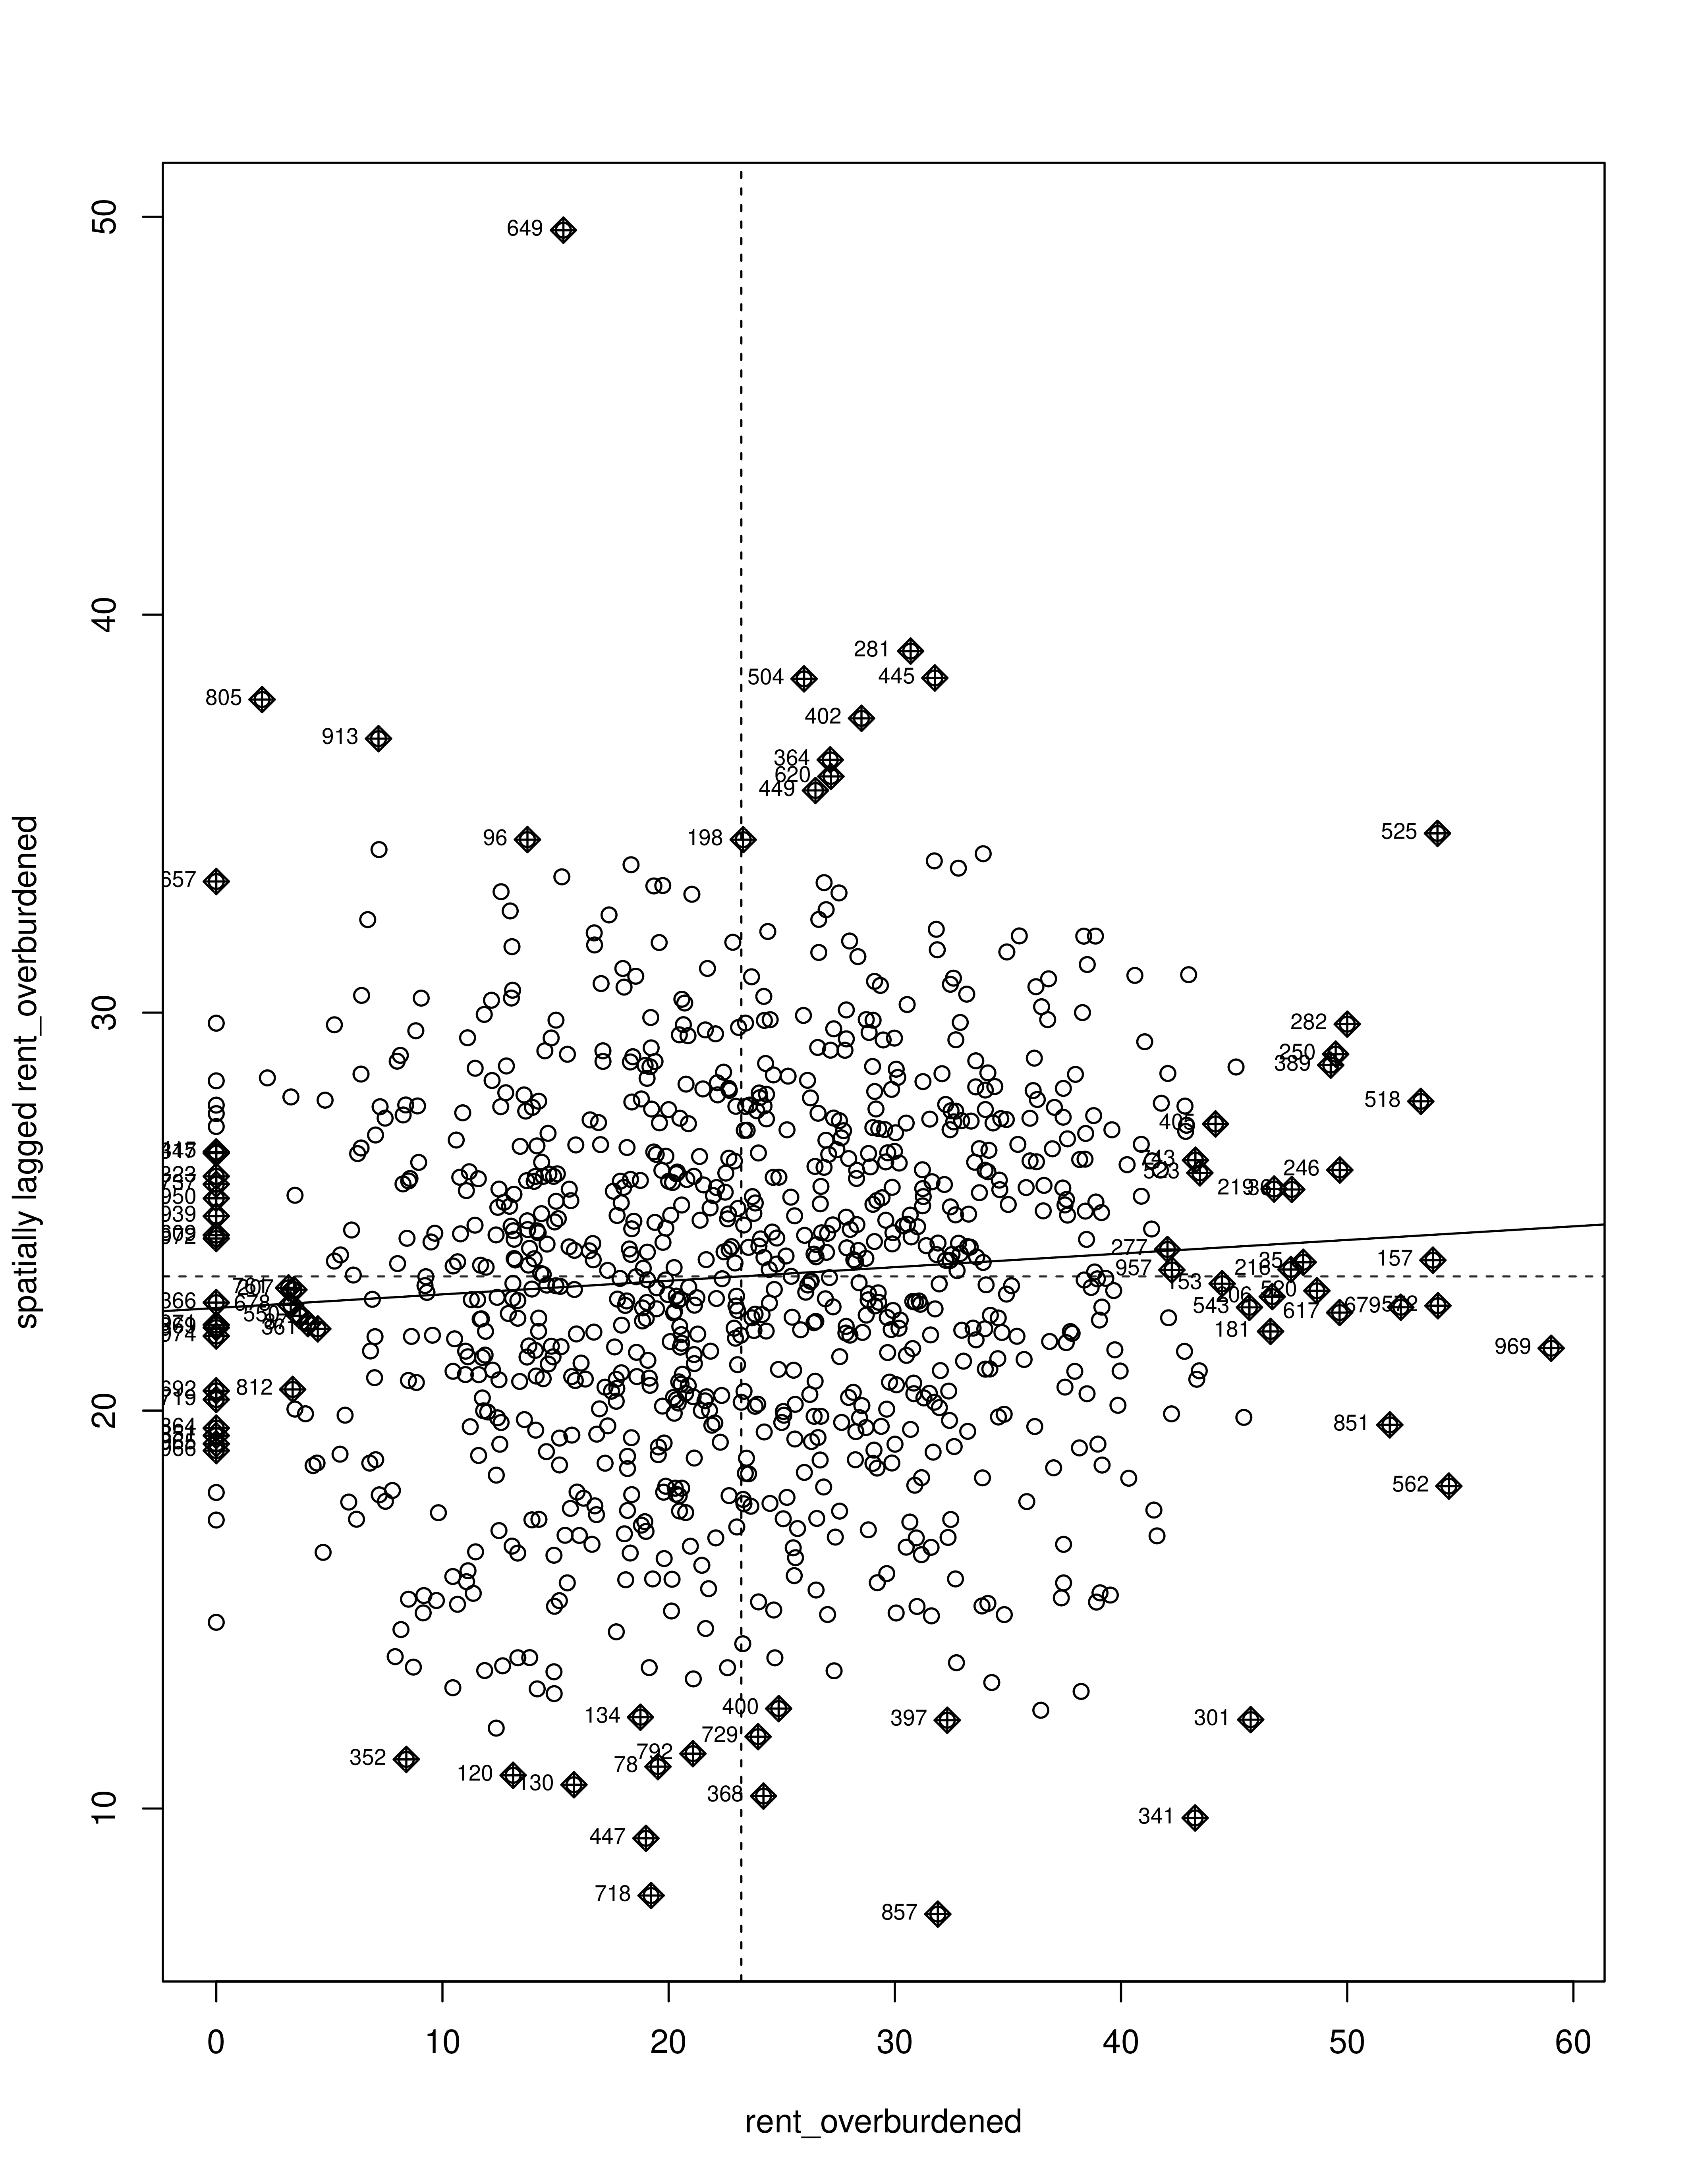
\includegraphics[scale=0.09]{Moran_rent_overburdened}
\end{figure}





\begin{table}[!htbp] \centering 
\caption{Spatial Lag Model (rent-overburdened ~ selected variables)} 
\label{} 
\begin{tabular}{@{\extracolsep{5pt}}lc} 
\\[-1.8ex]\hline 
\hline \\[-1.8ex] 
& \multicolumn{1}{c}{\textit{Dependent variable:}} \\ 
\cline{2-2} 
\\[-1.8ex] & rent\_overburdened \\ 
\hline \\[-1.8ex] 
log\_BART\_dist & 1.310$^{***}$ \\ 
& (0.330) \\ 
& \\ 
log\_CBD\_dist & 0.833$^{**}$ \\ 
& (0.339) \\ 
& \\ 
coastal\_tracts\_dummy & $-$3.012 \\ 
& (2.079) \\ 
& \\ 
percent\_non\_white & 0.022 \\ 
& (0.016) \\ 
& \\ 
log\_MHI & $-$12.037$^{***}$ \\ 
& (0.736) \\ 
& \\ 
percent\_airbnb\_all\_rentals & 0.051$^{***}$ \\ 
& (0.018) \\ 
& \\ 
Constant & 148.430$^{***}$ \\ 
& (8.455) \\ 
& \\ 
\hline \\[-1.8ex] 
Observations & 975 \\ 
Log Likelihood & $-$3,552.350 \\ 
$\sigma^{2}$ & 85.540 \\ 
Akaike Inf. Crit. & 7,122.701 \\ 
Wald Test & 0.035 (df = 1) \\ 
LR Test & 0.037 (df = 1) \\ 
\hline 
\hline \\[-1.8ex] 
\textit{Note:}  & \multicolumn{1}{r}{$^{*}$p$<$0.1; $^{**}$p$<$0.05; $^{***}$p$<$0.01} \\ 
\end{tabular} 
\end{table} 



% Table created by stargazer v.5.2 by Marek Hlavac, Harvard University. E-mail: hlavac at fas.harvard.edu
% Date and time: Thu, May 24, 2018 - 09:10:52 PM
\begin{table}[!htbp] \centering 
  \caption{Spatial Error Model - rent-overburdened ~ selected variables} 
  \label{} 
  \begin{tabular}{@{\extracolsep{5pt}}lc} 
    \\[-1.8ex]\hline 
    \hline \\[-1.8ex] 
    & \multicolumn{1}{c}{\textit{Dependent variable:}} \\ 
    \cline{2-2} 
    \\[-1.8ex] & rent\_overburdened \\ 
    \hline \\[-1.8ex] 
    log\_BART\_dist & 1.308$^{***}$ \\ 
    & (0.329) \\ 
    & \\ 
    log\_CBD\_dist & 0.834$^{**}$ \\ 
    & (0.337) \\ 
    & \\ 
    coastal\_tracts\_dummy & $-$3.010 \\ 
    & (2.075) \\ 
    & \\ 
    percent\_non\_white & 0.022 \\ 
    & (0.016) \\ 
    & \\ 
    log\_MHI & $-$12.028$^{***}$ \\ 
    & (0.730) \\ 
    & \\ 
    percent\_airbnb\_all\_rentals & 0.051$^{***}$ \\ 
    & (0.018) \\ 
    & \\ 
    Constant & 148.129$^{***}$ \\ 
    & (8.194) \\ 
    & \\ 
    \hline \\[-1.8ex] 
    Observations & 975 \\ 
    Log Likelihood & $-$3,552.274 \\ 
    $\sigma^{2}$ & 85.520 \\ 
    Akaike Inf. Crit. & 7,122.548 \\ 
    Wald Test & 0.185 (df = 1) \\ 
    LR Test & 0.189 (df = 1) \\ 
    \hline 
    \hline \\[-1.8ex] 
    \textit{Note:}  & \multicolumn{1}{r}{$^{*}$p$<$0.1; $^{**}$p$<$0.05; $^{***}$p$<$0.01} \\ 
  \end{tabular} 
\end{table} 


% ===============================================================
% Analysis for log_median_rent begins below:



% Table created by stargazer v.5.2 by Marek Hlavac, Harvard University. E-mail: hlavac at fas.harvard.edu
% Date and time: Thu, May 24, 2018 - 09:13:58 PM
\begin{table}[!htbp] \centering 
  \caption{Regression - log-median-rent ~ selected variables} 
  \label{} 
  \begin{tabular}{@{\extracolsep{5pt}}lc} 
    \\[-1.8ex]\hline 
    \hline \\[-1.8ex] 
    & \multicolumn{1}{c}{\textit{Dependent variable:}} \\ 
    \cline{2-2} 
    \\[-1.8ex] & log\_median\_rent \\ 
    \hline \\[-1.8ex] 
    log\_BART\_dist & 0.031$^{***}$ \\ 
    & (0.010) \\ 
    & \\ 
    log\_CBD\_dist & 0.032$^{***}$ \\ 
    & (0.010) \\ 
    & \\ 
    coastal\_tracts\_dummy & $-$0.044 \\ 
    & (0.064) \\ 
    & \\ 
    percent\_non\_white & $-$0.001 \\ 
    & (0.0005) \\ 
    & \\ 
    log\_MHI & 0.237$^{***}$ \\ 
    & (0.023) \\ 
    & \\ 
    percent\_airbnb\_all\_rentals & 0.0004 \\ 
    & (0.001) \\ 
    & \\ 
    Constant & 4.437$^{***}$ \\ 
    & (0.254) \\ 
    & \\ 
    \hline \\[-1.8ex] 
    Observations & 975 \\ 
    R$^{2}$ & 0.223 \\ 
    Adjusted R$^{2}$ & 0.219 \\ 
    Residual Std. Error & 0.286 (df = 968) \\ 
    F Statistic & 46.394$^{***}$ (df = 6; 968) \\ 
    \hline 
    \hline \\[-1.8ex] 
    \textit{Note:}  & \multicolumn{1}{r}{$^{*}$p$<$0.1; $^{**}$p$<$0.05; $^{***}$p$<$0.01} \\ 
  \end{tabular} 
\end{table} 


% Table created by stargazer v.5.2 by Marek Hlavac, Harvard University. E-mail: hlavac at fas.harvard.edu
% Date and time: Thu, May 24, 2018 - 09:15:22 PM
\begin{table}[!htbp] \centering 
  \caption{Variance Inflation Factor - Test for Multicolinearity} 
  \label{} 
  \hspace*{-2.5cm}
  \begin{tabular}{@{\extracolsep{5pt}} cccccc} 
    \\[-1.8ex]\hline 
    \hline \\[-1.8ex] 
    log\_BART\_dist & log\_CBD\_dist & coastal\_tracts\_dummy & percent\_non\_white & log\_MHI & percent\_airbnb\_all\_rentals \\ 
    \hline \\[-1.8ex] 
    $1.534$ & $1.494$ & $1.039$ & $1.401$ & $1.441$ & $1.164$ \\ 
    \hline \\[-1.8ex] 
  \end{tabular} 
\end{table} 

% Table created by stargazer v.5.2 by Marek Hlavac, Harvard University. E-mail: hlavac at fas.harvard.edu
% Date and time: Thu, May 24, 2018 - 09:17:49 PM
\begin{table}[!htbp] \centering 
  \caption{Spatial Lag model - log-median-rent ~ selected variables} 
  \label{} 
  \begin{tabular}{@{\extracolsep{5pt}}lc} 
    \\[-1.8ex]\hline 
    \hline \\[-1.8ex] 
    & \multicolumn{1}{c}{\textit{Dependent variable:}} \\ 
    \cline{2-2} 
    \\[-1.8ex] & log\_median\_rent \\ 
    \hline \\[-1.8ex] 
    log\_BART\_dist & 0.031$^{***}$ \\ 
    & (0.010) \\ 
    & \\ 
    log\_CBD\_dist & 0.031$^{***}$ \\ 
    & (0.010) \\ 
    & \\ 
    coastal\_tracts\_dummy & $-$0.032 \\ 
    & (0.064) \\ 
    & \\ 
    percent\_non\_white & $-$0.001 \\ 
    & (0.0005) \\ 
    & \\ 
    log\_MHI & 0.228$^{***}$ \\ 
    & (0.023) \\ 
    & \\ 
    percent\_airbnb\_all\_rentals & 0.0004 \\ 
    & (0.001) \\ 
    & \\ 
    Constant & 3.478$^{***}$ \\ 
    & (0.411) \\ 
    & \\ 
    \hline \\[-1.8ex] 
    Observations & 975 \\ 
    Log Likelihood & $-$154.626 \\ 
    $\sigma^{2}$ & 0.080 \\ 
    Akaike Inf. Crit. & 327.252 \\ 
    Wald Test & 9.424$^{***}$ (df = 1) \\ 
    LR Test & 9.518$^{***}$ (df = 1) \\ 
    \hline 
    \hline \\[-1.8ex] 
    \textit{Note:}  & \multicolumn{1}{r}{$^{*}$p$<$0.1; $^{**}$p$<$0.05; $^{***}$p$<$0.01} \\ 
  \end{tabular} 
\end{table} 




% Table created by stargazer v.5.2 by Marek Hlavac, Harvard University. E-mail: hlavac at fas.harvard.edu
% Date and time: Thu, May 24, 2018 - 09:51:30 PM
\begin{table}[!htbp] \centering 
  \caption{Spatial Error Model - log-median-rent ~ selected variables} 
  \label{} 
  \begin{tabular}{@{\extracolsep{5pt}}lc} 
    \\[-1.8ex]\hline 
    \hline \\[-1.8ex] 
    & \multicolumn{1}{c}{\textit{Dependent variable:}} \\ 
    \cline{2-2} 
    \\[-1.8ex] & log\_median\_rent \\ 
    \hline \\[-1.8ex] 
    log\_BART\_dist & 0.032$^{***}$ \\ 
    & (0.010) \\ 
    & \\ 
    log\_CBD\_dist & 0.032$^{***}$ \\ 
    & (0.011) \\ 
    & \\ 
    coastal\_tracts\_dummy & $-$0.026 \\ 
    & (0.064) \\ 
    & \\ 
    percent\_non\_white & $-$0.001 \\ 
    & (0.001) \\ 
    & \\ 
    log\_MHI & 0.229$^{***}$ \\ 
    & (0.023) \\ 
    & \\ 
    percent\_airbnb\_all\_rentals & 0.0005 \\ 
    & (0.001) \\ 
    & \\ 
    Constant & 4.529$^{***}$ \\ 
    & (0.257) \\ 
    & \\ 
    \hline \\[-1.8ex] 
    Observations & 975 \\ 
    Log Likelihood & $-$156.409 \\ 
    $\sigma^{2}$ & 0.080 \\ 
    Akaike Inf. Crit. & 330.817 \\ 
    Wald Test & 6.318$^{**}$ (df = 1) \\ 
    LR Test & 5.952$^{**}$ (df = 1) \\ 
    \hline 
    \hline \\[-1.8ex] 
    \textit{Note:}  & \multicolumn{1}{r}{$^{*}$p$<$0.1; $^{**}$p$<$0.05; $^{***}$p$<$0.01} \\ 
  \end{tabular} 
\end{table} 


% Table created by stargazer v.5.2 by Marek Hlavac, Harvard University. E-mail: hlavac at fas.harvard.edu
% Date and time: Thu, May 24, 2018 - 09:56:32 PM
\begin{table}[!htbp] \centering 
  \caption{Variance Inflation Factor - test for MC} 
  \label{}
  \hspace*{-4.5cm} 
  \begin{tabular}{@{\extracolsep{5pt}} cccccc} 
    \\[-1.8ex]\hline 
    \hline \\[-1.8ex] 
    log\_BART\_dist & log\_CBD\_dist & coastal\_tracts\_dummy & percent\_non\_white & log\_MHI & percent\_airbnb\_active\_rentals \\ 
    \hline \\[-1.8ex] 
    $1.534$ & $1.475$ & $1.039$ & $1.401$ & $1.422$ & $1.140$ \\ 
    \hline \\[-1.8ex] 
  \end{tabular} 
\end{table}


% Table created by stargazer v.5.2 by Marek Hlavac, Harvard University. E-mail: hlavac at fas.harvard.edu
% Date and time: Thu, May 24, 2018 - 09:57:44 PM
\begin{table}[!htbp] \centering 
  \caption{OLS Regression - log-median-rent ~ selected variables} 
  \label{} 
  \begin{tabular}{@{\extracolsep{5pt}}lc} 
    \\[-1.8ex]\hline 
    \hline \\[-1.8ex] 
    & \multicolumn{1}{c}{\textit{Dependent variable:}} \\ 
    \cline{2-2} 
    \\[-1.8ex] & log\_median\_rent \\ 
    \hline \\[-1.8ex] 
    Xlog\_BART\_dist & 1.538$^{***}$ \\ 
    & (0.408) \\ 
    & \\ 
    Xlog\_CBD\_dist & 2.365$^{***}$ \\ 
    & (0.416) \\ 
    & \\ 
    Xcoastal\_tracts\_dummy & $-$4.574$^{*}$ \\ 
    & (2.567) \\ 
    & \\ 
    Xpercent\_non\_white & 0.046$^{**}$ \\ 
    & (0.020) \\ 
    & \\ 
    Xlog\_MHI & $-$16.541$^{***}$ \\ 
    & (0.922) \\ 
    & \\ 
    Xpercent\_airbnb\_active\_rentals & 0.041$^{**}$ \\ 
    & (0.018) \\ 
    & \\ 
    XSchool\_district\_quality & 0.078 \\ 
    & (0.103) \\ 
    & \\ 
    Constant & 212.809$^{***}$ \\ 
    & (10.289) \\ 
    & \\ 
    \hline \\[-1.8ex] 
    Observations & 975 \\ 
    R$^{2}$ & 0.327 \\ 
    Adjusted R$^{2}$ & 0.322 \\ 
    Residual Std. Error & 11.416 (df = 967) \\ 
    F Statistic & 67.018$^{***}$ (df = 7; 967) \\ 
    \hline 
    \hline \\[-1.8ex] 
    \textit{Note:}  & \multicolumn{1}{r}{$^{*}$p$<$0.1; $^{**}$p$<$0.05; $^{***}$p$<$0.01} \\ 
  \end{tabular} 
\end{table}


\begin{figure}[!htbp]
  \caption{Moran's I test for spatial autocorrelation}
  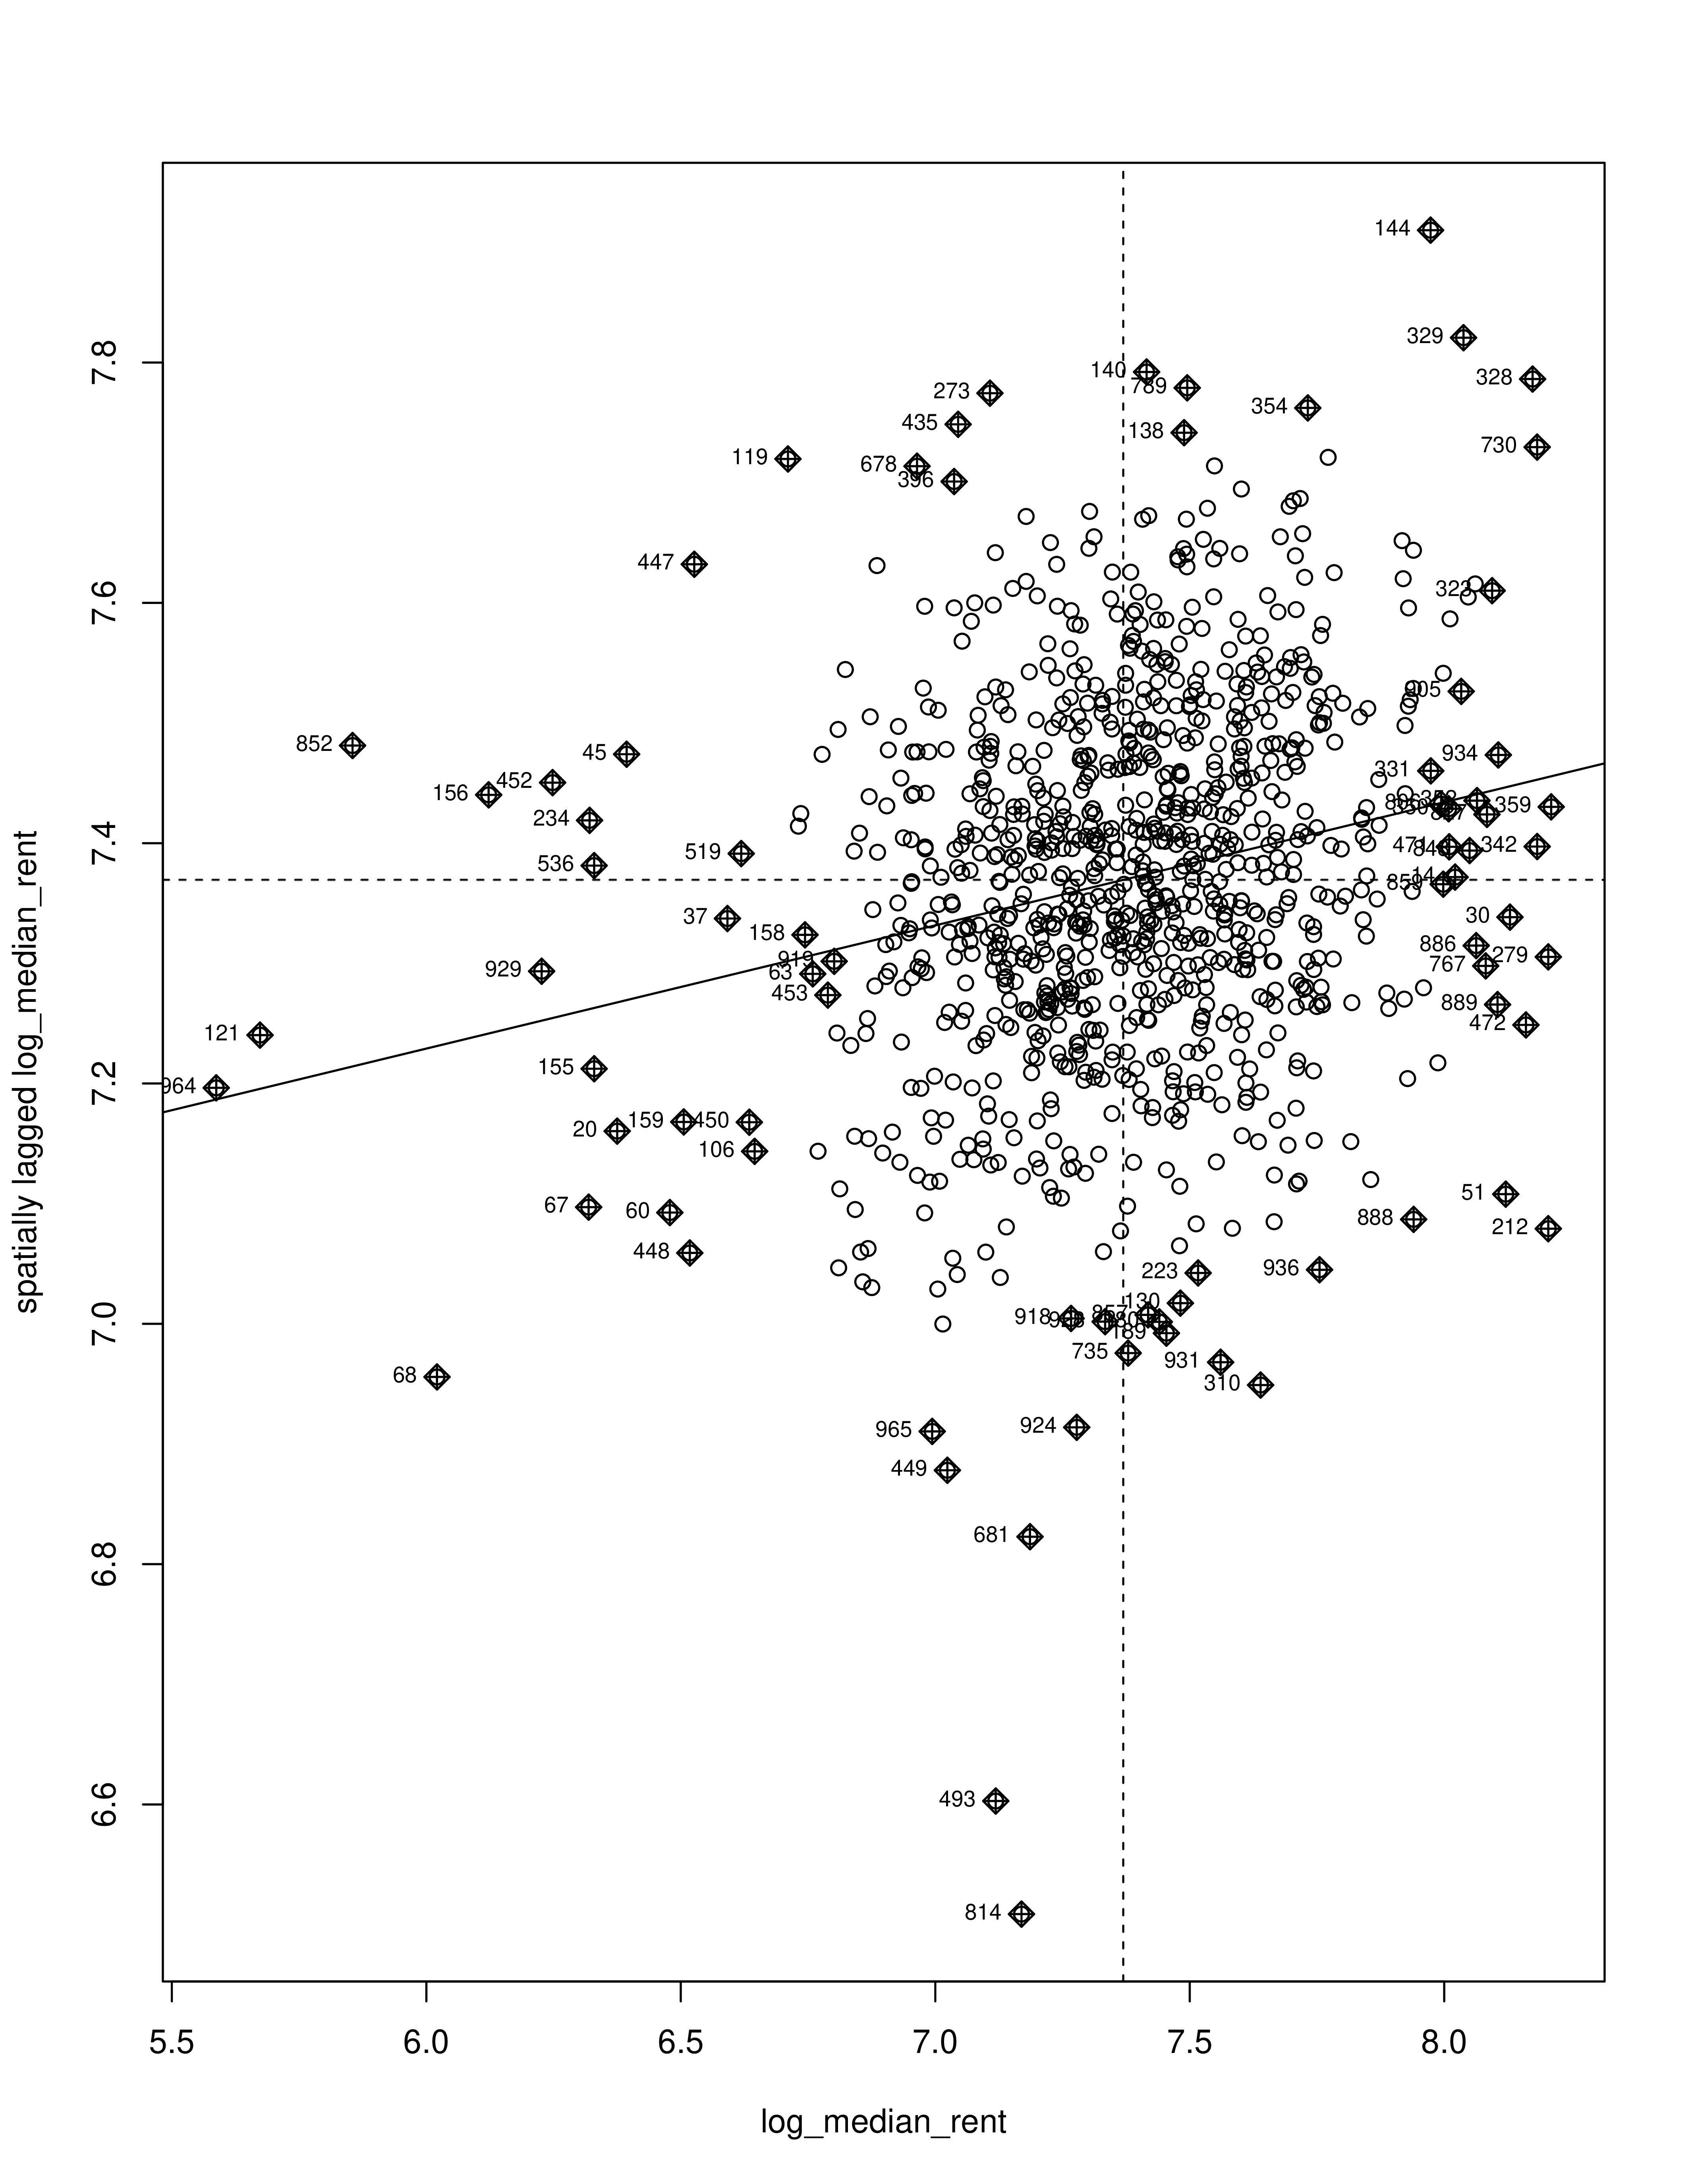
\includegraphics[scale=0.09]{Moran_active_rentals}
\end{figure}


% Table created by stargazer v.5.2 by Marek Hlavac, Harvard University. E-mail: hlavac at fas.harvard.edu
% Date and time: Thu, May 24, 2018 - 10:00:35 PM
\begin{table}[!htbp] \centering 
  \caption{Spatial Lag Model - log median rent - selected variables (active rentals)} 
  \label{} 
  \begin{tabular}{@{\extracolsep{5pt}}lc} 
    \\[-1.8ex]\hline 
    \hline \\[-1.8ex] 
    & \multicolumn{1}{c}{\textit{Dependent variable:}} \\ 
    \cline{2-2} 
    \\[-1.8ex] & log\_median\_rent \\ 
    \hline \\[-1.8ex] 
    log\_BART\_dist & 0.031$^{***}$ \\
    & (0.010) \\ 
    & \\ 
    log\_CBD\_dist & 0.029$^{***}$ \\ 
    & (0.010) \\ 
    & \\ 
    coastal\_tracts\_dummy & $-$0.032 \\ 
    & (0.064) \\ 
    & \\ 
    percent\_non\_white & $-$0.001 \\ 
    & (0.0005) \\ 
    & \\ 
    log\_MHI & 0.230$^{***}$ \\ 
    & (0.022) \\ 
    & \\ 
    percent\_airbnb\_active\_rentals & 0.0001 \\ 
    & (0.0005) \\ 
    & \\ 
    Constant & 3.464$^{***}$ \\ 
    & (0.410) \\ 
    & \\ 
    \hline \\[-1.8ex] 
    Observations & 975 \\ 
    Log Likelihood & $-$154.873 \\ 
    $\sigma^{2}$ & 0.080 \\ 
    Akaike Inf. Crit. & 327.745 \\ 
    Wald Test & 9.461$^{***}$ (df = 1) \\ 
    LR Test & 9.556$^{***}$ (df = 1) \\ 
    \hline 
    \hline \\[-1.8ex] 
    \textit{Note:}  & \multicolumn{1}{r}{$^{*}$p$<$0.1; $^{**}$p$<$0.05; $^{***}$p$<$0.01} \\ 
  \end{tabular} 
\end{table} 


% Table created by stargazer v.5.2 by Marek Hlavac, Harvard University. E-mail: hlavac at fas.harvard.edu
% Date and time: Thu, May 24, 2018 - 10:01:59 PM
\begin{table}[!htbp] \centering 
  \caption{Spatial Error Model - log-median-rent with selected variables (active rentals)} 
  \label{} 
  \begin{tabular}{@{\extracolsep{5pt}}lc} 
    \\[-1.8ex]\hline 
    \hline \\[-1.8ex] 
    & \multicolumn{1}{c}{\textit{Dependent variable:}} \\ 
    \cline{2-2} 
    \\[-1.8ex] & log\_median\_rent \\ 
    \hline \\[-1.8ex] 
    log\_BART\_dist & 0.032$^{***}$ \\ 
    & (0.010) \\ 
    & \\ 
    log\_CBD\_dist & 0.030$^{***}$ \\ 
    & (0.011) \\ 
    & \\ 
    coastal\_tracts\_dummy & $-$0.026 \\ 
    & (0.064) \\ 
    & \\ 
    percent\_non\_white & $-$0.001 \\ 
    & (0.001) \\ 
    & \\ 
    log\_MHI & 0.231$^{***}$ \\ 
    & (0.023) \\ 
    & \\ 
    percent\_airbnb\_active\_rentals & 0.0001 \\ 
    & (0.0005) \\ 
    & \\ 
    Constant & 4.514$^{***}$ \\ 
    & (0.257) \\ 
    & \\ 
    \hline \\[-1.8ex] 
    Observations & 975 \\ 
    Log Likelihood & $-$156.717 \\ 
    $\sigma^{2}$ & 0.081 \\ 
    Akaike Inf. Crit. & 331.433 \\ 
    Wald Test & 6.230$^{**}$ (df = 1) \\ 
    LR Test & 5.868$^{**}$ (df = 1) \\ 
    \hline 
    \hline \\[-1.8ex] 
    \textit{Note:}  & \multicolumn{1}{r}{$^{*}$p$<$0.1; $^{**}$p$<$0.05; $^{***}$p$<$0.01} \\ 
  \end{tabular} 
\end{table}




% Table created by stargazer v.5.2 by Marek Hlavac, Harvard University. E-mail: hlavac at fas.harvard.edu
% Date and time: Thu, May 24, 2018 - 10:06:29 PM
\begin{table}[!htbp] \centering 
  \caption{Regression - rent-hourly wage and selected variables} 
  \label{} 
  \begin{tabular}{@{\extracolsep{5pt}}lc} 
    \\[-1.8ex]\hline 
    \hline \\[-1.8ex] 
    & \multicolumn{1}{c}{\textit{Dependent variable:}} \\ 
    \cline{2-2} 
    \\[-1.8ex] & rent\_hourly\_wage \\ 
    \hline \\[-1.8ex] 
    log\_BART\_dist & 0.879$^{***}$ \\ 
    & (0.252) \\ 
    & \\ 
    log\_CBD\_dist & $-$3.266$^{***}$ \\ 
    & (0.259) \\ 
    & \\ 
    coastal\_tracts\_dummy & 0.585 \\ 
    & (1.589) \\ 
    & \\ 
    percent\_non\_white & 0.047$^{***}$ \\ 
    & (0.012) \\ 
    & \\ 
    log\_MHI & 2.441$^{***}$ \\ 
    & (0.560) \\ 
    & \\ 
    percent\_airbnb\_all\_rentals & 0.012 \\ 
    & (0.014) \\ 
    & \\ 
    Constant & $-$0.807 \\ 
    & (6.285) \\ 
    & \\ 
    \hline \\[-1.8ex] 
    Observations & 975 \\ 
    R$^{2}$ & 0.173 \\ 
    Adjusted R$^{2}$ & 0.167 \\ 
    Residual Std. Error & 7.067 (df = 968) \\ 
    F Statistic & 33.657$^{***}$ (df = 6; 968) \\ 
    \hline 
    \hline \\[-1.8ex] 
    \textit{Note:}  & \multicolumn{1}{r}{$^{*}$p$<$0.1; $^{**}$p$<$0.05; $^{***}$p$<$0.01} \\ 
  \end{tabular} 
\end{table}



% Table created by stargazer v.5.2 by Marek Hlavac, Harvard University. E-mail: hlavac at fas.harvard.edu
% Date and time: Thu, May 24, 2018 - 10:08:13 PM
\begin{table}[!htbp] \centering 
  \caption{Variance Inflation Matrix - Rent hourly wage with selected variables} 
  \label{}
  \hspace*{-4.5cm}
  \begin{tabular}{@{\extracolsep{5pt}} cccccc} 
    \\[-1.8ex]\hline 
    \hline \\[-1.8ex] 
    log\_BART\_dist & log\_CBD\_dist & coastal\_tracts\_dummy & percent\_non\_white & log\_MHI & percent\_airbnb\_all\_rentals \\ 
    \hline \\[-1.8ex] 
    $1.534$ & $1.494$ & $1.039$ & $1.401$ & $1.441$ & $1.164$ \\ 
    \hline \\[-1.8ex] 
  \end{tabular} 
\end{table} 

















\end{document}
